\graphicspath{{figures/results}}
\section{Results} \label{sec:results}
% Summary of Results I want to show:
% Need a table with all of the parameter values varied (DONE!)
% Would *like* to have a torus only parameter estimation to show, then basically just keeping the "torus only section". Justification: showing that just a torus is not sufficient.
% Then adding the "we varied all of the parameters" section, splitting up by priors and no priors. Add the priors corner plots for both cases. Justification: we will discuss further the priors choice in the discussion.
% Tables can have the different sp and clfrac combinations. Justification: we will then show in the discussion that one of these combos maybe is better than the others?
% Can show lightcurves of the best fits (priors param combos in one plot no priors param combos in another plot). Justification: we discuss the degeneracy of our model.


%Order:
% Torus only parameter set table
% Torus only corner plot and or table
% All params parameter set table
% All params corner plot for no priors
% All params corner plot for priors
% sp and clfrac posterior table 
\begin{table}
    \cite{}
    \caption{Parameter values used to construct the model grids in this work. Parameter values represent points on a regular grid with no gaps, ie. all possible combinations of parameters are evaluated. }
    \label{tab:params}
    \centering
    \begin{tabular}[c]{c@{\hskip 0.1in}c@{\hskip 0.1in}c@{\hskip 0.1in}c@{\hskip 0.1in}c@{\hskip 0.1in}c@{\hskip 0.1in}c@{\hskip 0.1in}c}
        \hline
        \hline
        Parameter & Torus Only & Torus \& Polar\\
        \hline
        \hline
        \Y&10, 25, 50, 75, 100, 500&2, 5, 10, 25, 50\\
        \hline
        \sig&5, 10, 30, 45&2, 5, 10, 20\\
        \hline
        \p&-2, -1, 0, 1, 2&-1, 0, 1, 2\\
        \hline
        \vff&-1, -2, -3, -4&-1, -2, -3, -4\\
        \hline
        \inc&0, 30, 45, 60, 90&0, 30, 45, 60, 75\\
        \hline
        \soft&1.0 (iso), 0.1 (aniso)&1.0, 0.1\\
        \hline
        \Ypol&--&5, 50, 100\\
        \hline
        \sigpol&--&2, 10, 20\\
        \hline
        \ppol&--& -1, 0, 1, 2\\
        \hline
        \vffpol&--&-1, -2, -3, -4\\
        \hline
        \open&--&10, 25, 40\\
        \hline
        \clfrac&--&0.333, 0.667\\
        \hline
        numclouds&50000&100000
    \end{tabular}
\end{table}

\par As discussed in Section~\ref{sec:codereview}, TORMAC is able to model the IR response from an AGN, producing the response IR light curve from the input optical light curve. In this section we focus on the resulting parameter estimations from a variety of modeled dust cloud distributions to the observed light curves. We begin by evaluating a regular grid \zach{I define "regular grid" only below} of models which only vary the parameters in the torus dust distribution (\Y, \sig, \p, \vff, as well as \inc). Because we know that NGC 3783 likely has a polar dust distribution, we also construct a model grid which jointly simulates a torus and polar dust distribution, again varying \Y, \sig, \p, \vff, \& \inc, but also varying \Ypol, \sigpol, \ppol, \vffpol, and \open. For each of our model grids, we evaluate both isotropic (\soft $= 1.0$) and anisotropic (\soft $= 0.1$) illumination cases. In all cases, we generate TORMAC simulated response light curves in both the H and K bands.

% After evaluating the model grid, we use Dynesty’s dynamic nested‑sampling algorithm, which draws parameters from a uniform prior and computes their corresponding likelihood values. To sample light curves continuously within the prior space, we linearly interpolate between adjacent TORMAC models within our grid. To compute the likelihood value of a given sample's parameter values, we adjust the magnitude of the response by a monochromatic scaling factor which maximizes the gaussian likelihood to the observed IR response, then calculate the gaussian likelihood to said response. Across both grids and in all cases presented in this work, we use the same configuration of Dynesty dynamic nested sampling algorithm, with 2000 live points and a target of 600000 posterior samples as our stopping criterion. 

%Expanded of above
\par After evaluating the model grid, we use Dynesty’s dynamic nested‑sampling algorithm, which draws parameters from a uniform prior and computes their corresponding likelihood values. We need to sample light curves continuously within the maximum and minimum bounds of each parameter our grid (the prior space). To do this, we linearly interpolate between adjacent TORMAC models in our grid. This is an approximation which we assess in Section~\ref{sec:discussion}. To calculate the likelihood, we first modify the interpolated response light curves by multiplicatively scaling both light curves by a single scaling factor which maximizes the sample's joint gaussian likelihood to both the H and K band IR observed response light curves. We then jointly calculate the gaussian likelihood to the observed H and K band IR response light curves of NGC3783. Across all grids and cases presented in this work, we use the same configuration of Dynesty dynamic nested sampling algorithm. We use a Dynesty configuration with 2000 live points and a target of 600000 posterior samples as our stopping criterion. 


\subsection{Torus Only Models} %Grid 1
\label{sec:torus_only_models}

\begin{figure}
 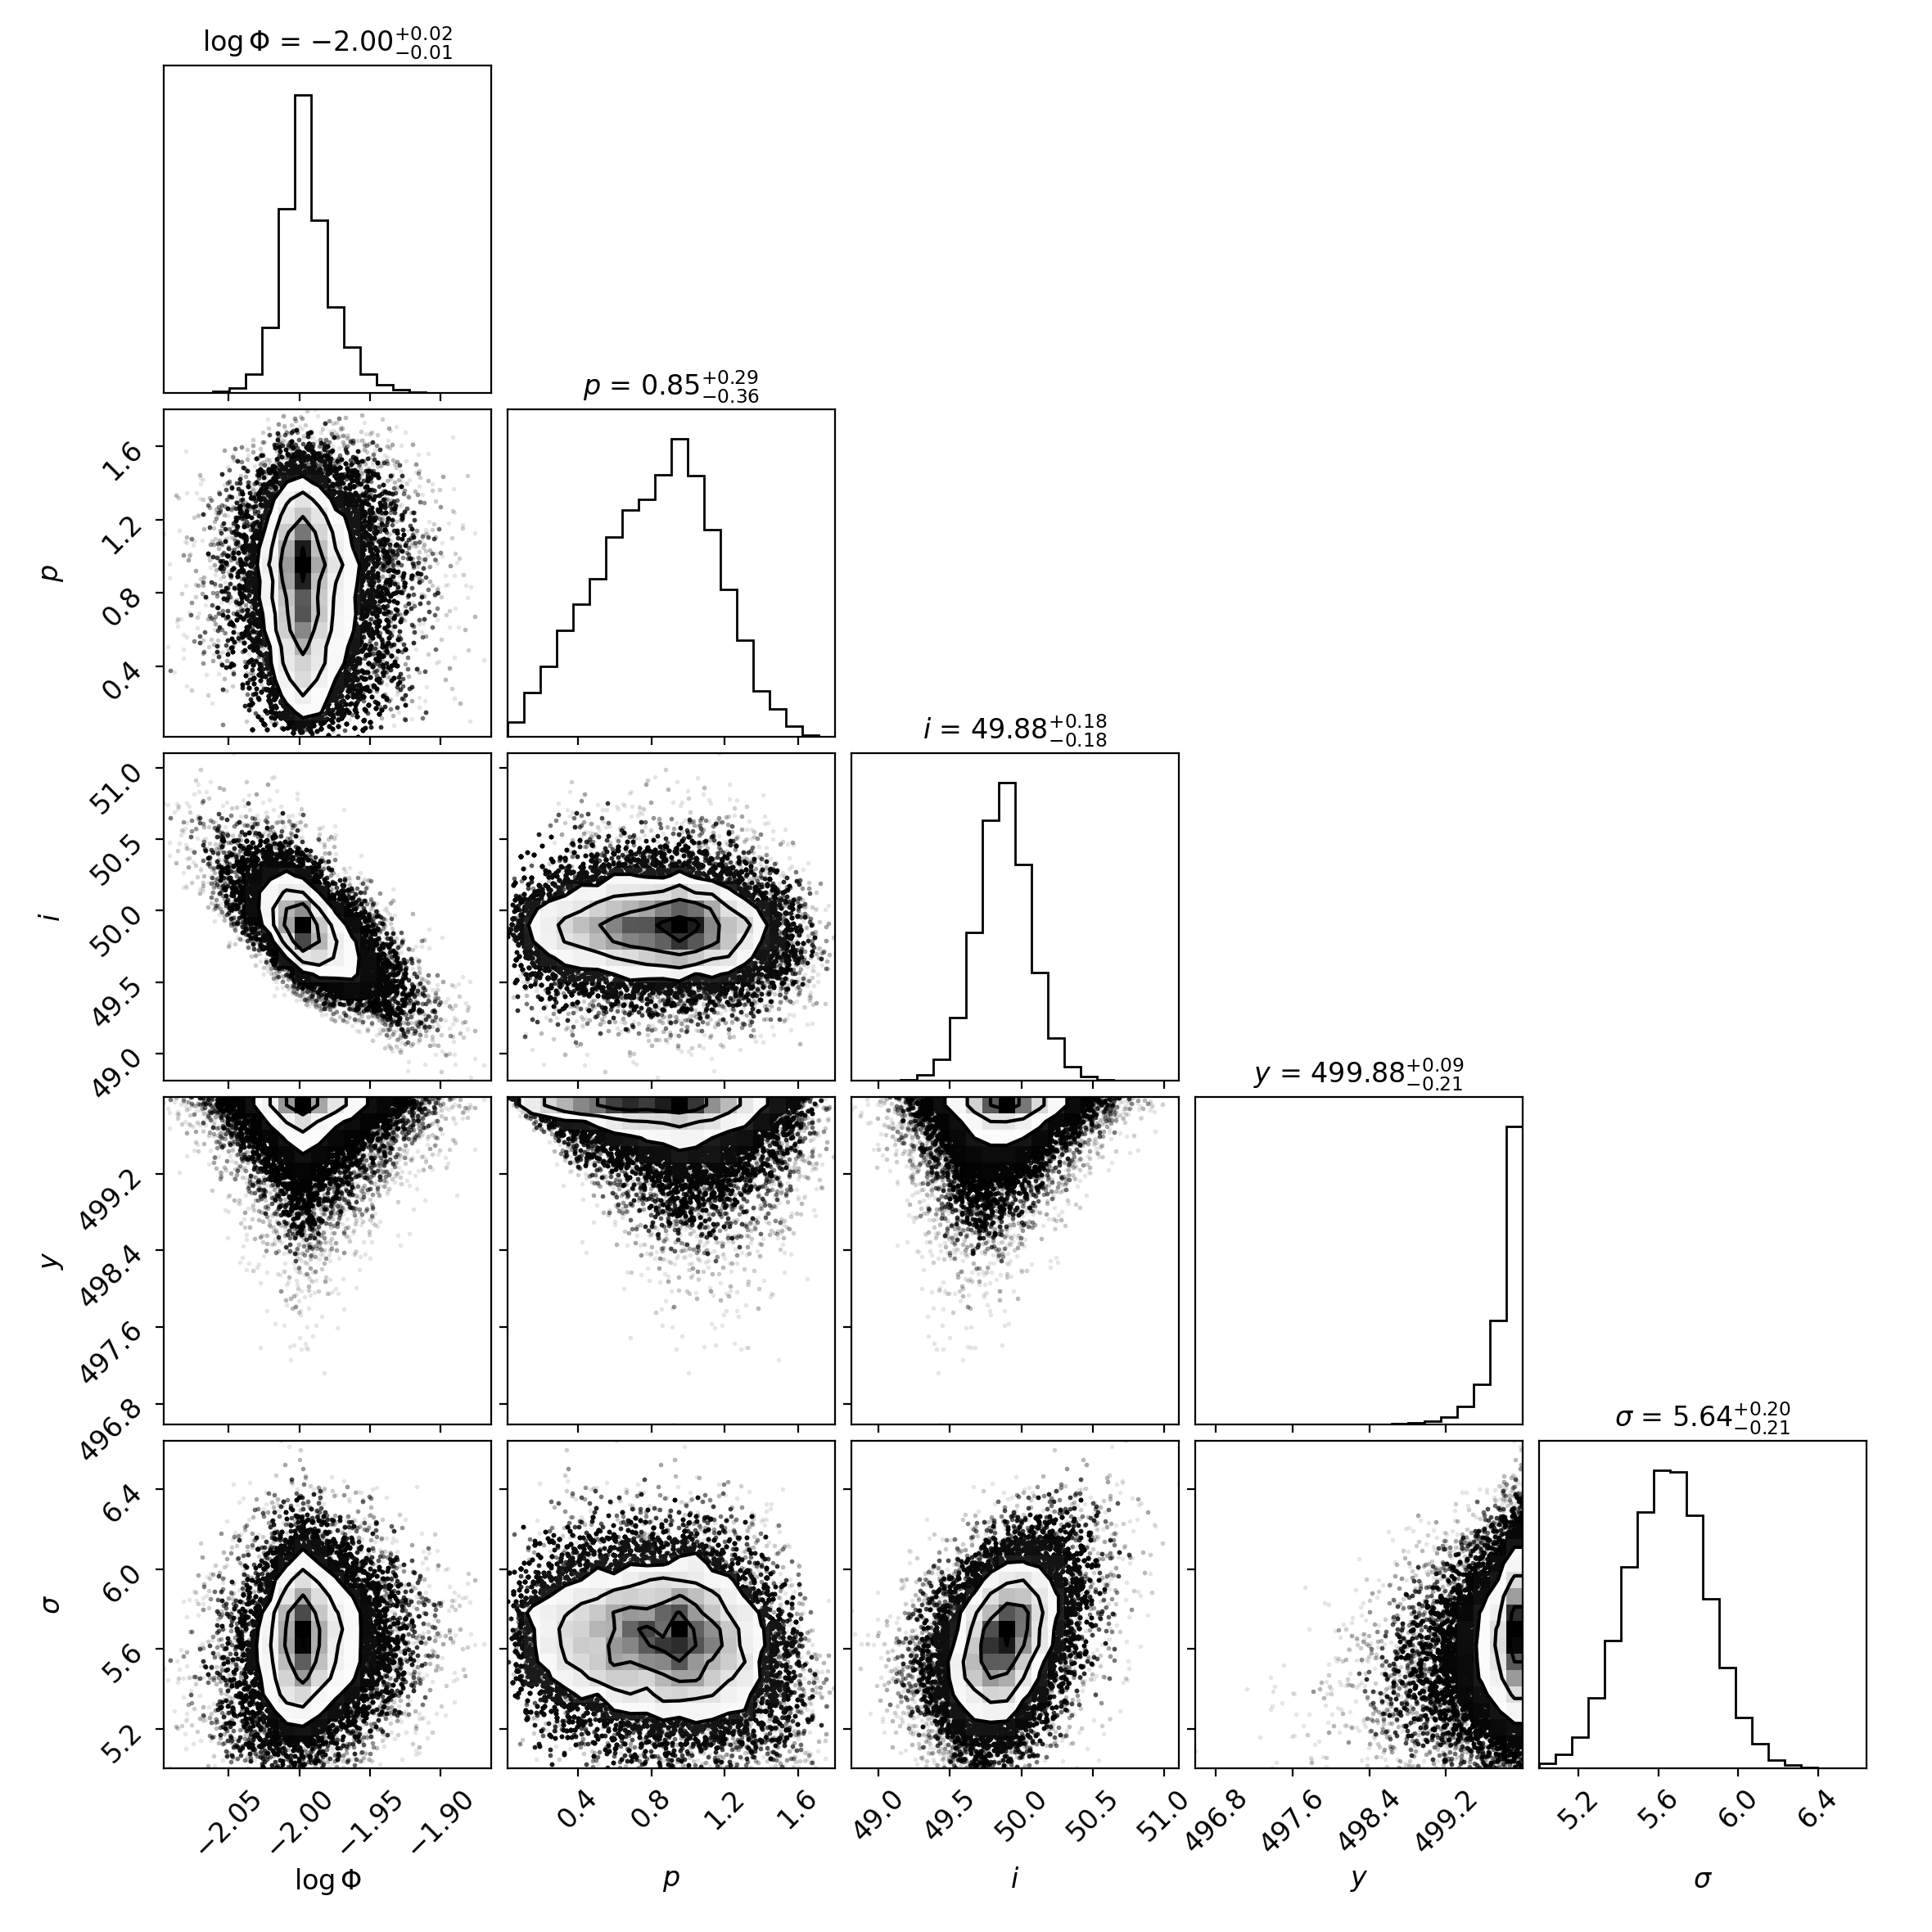
\includegraphics[scale=0.28]{figures/results/torus_only_corner_plots/dynesty_0.1_1.0__corner.png}
 \caption{Estimated posterior distributions of directly fitted parameters from the torus only model grid with \soft $=0.1$. 1-dimensional posterior distributions for the parameters \vff, \p, \i, \Y, and \sig lie on the diagonal, with the indicated value above each distribution corresponding to the maximum of the posterior distribution in that dimension. 2-dimensional posterior distributions for all combinations of parameters are shown in the lower triangle. The contours enclose the 0.5, 1, and 2 $\sigma$ regions of the posterior distribution. To avoid over crowding of points in the 2-dimensional posteriors, the shade of the region enclosed by the 2 $\sigma$ contour indicates the relative density of posterior samples.}
 \label{fig:tonlynopriorsparams}
\end{figure}

\par AGN circumnuclear dust has typically been modeled as a single compact disk component \zach{cite?}. We investigate if a single torus component is sufficient to model the observed IR light curves of NGC 3783 \zach{last two sentences actually go in intro?}. The geometric parameters of the torus (\Y, \sig, \inc, and \soft) as well as the structural parameters (\p and \vff) were varied independently, such that all possible combinations of the parameter values are sampled, herein referred to as a "regular grid". The model grid is finely sampled over these parameters (relative to the torus + polar grid), with a complete set of parameter values enumerated in Table~\ref{tab:params}. 

\par For both the anisotropic and isotropic illumination cases, we separately performed dynamic nested sampling using Dynesty. This was done to distinguish the influence from the type of illumination of the dust distribution from the rest of the parameters. We find that the [isotropic, anisotropic - ally illuminated] torus only model grid better describes the observed H and K band light curves of NGC3783, with a reduced statistic of [calculate and insert the reduced statistic] for the isotropic and anisotropic grids respectively. However, both of these model grids are a generally poor description of the data. The posterior distribution estimated from the anisotropic model grid are shown in Figure~\ref{fig:tonlynopriorsparams}. For the posterior distributions presented in this work, we choose to visualize both the 1-dimensional (along the diagonal) and 2-dimensional (in the lower triangle) posterior distributions. The 1-dimensional posterior distributions represent the posterior of each parameter varied in the torus only model grid (\vff, \p, \inc, \Y, \sig), with the value listed above each panel corresponding to the maximum of the posterior distribution for that given parameter. The 2-dimensional posterior distributions show the relationship between combinations of parameters. When a parameter or combination of parameters is well constrained, the posterior distribution for that parameter or combination of parameters will be roughly that of a gaussian, such as is the case for \inc, \sig, and the combination of \inc and \sig in the anisotropic illumination case of the torus only model grid. \inc and \vff are related, indicated by the skew present in the 2-dimensional posterior. This generally indicates that models with a closer to face on inclination are better supported when a greater fraction of the torus' volume contains clouds than for higher inclinations. \Y is not constrained in the torus only model grid with anisotropic illumination, indicated by the peak posterior value being very close to the edge of the posterior volume (\Y $= 500$), and the posterior distribution not being close to zero at the edge of the posterior volume. With the notable exception of \Y, all other parameters are constrained. \p is relatively weakly constrained, indicating that models with more centrally concentrated clouds and models with clouds concentrated at larger radii are able to describe the infrared response of NGC3783 nearly equally as well. For this set of models, NGC3783's infared response is best modeled by a moderately inclined, angularly thin, radially thick torus with roughly 1\% of the torus' volume containing clouds.

\subsubsection{Measured Variables}

\begin{figure}
 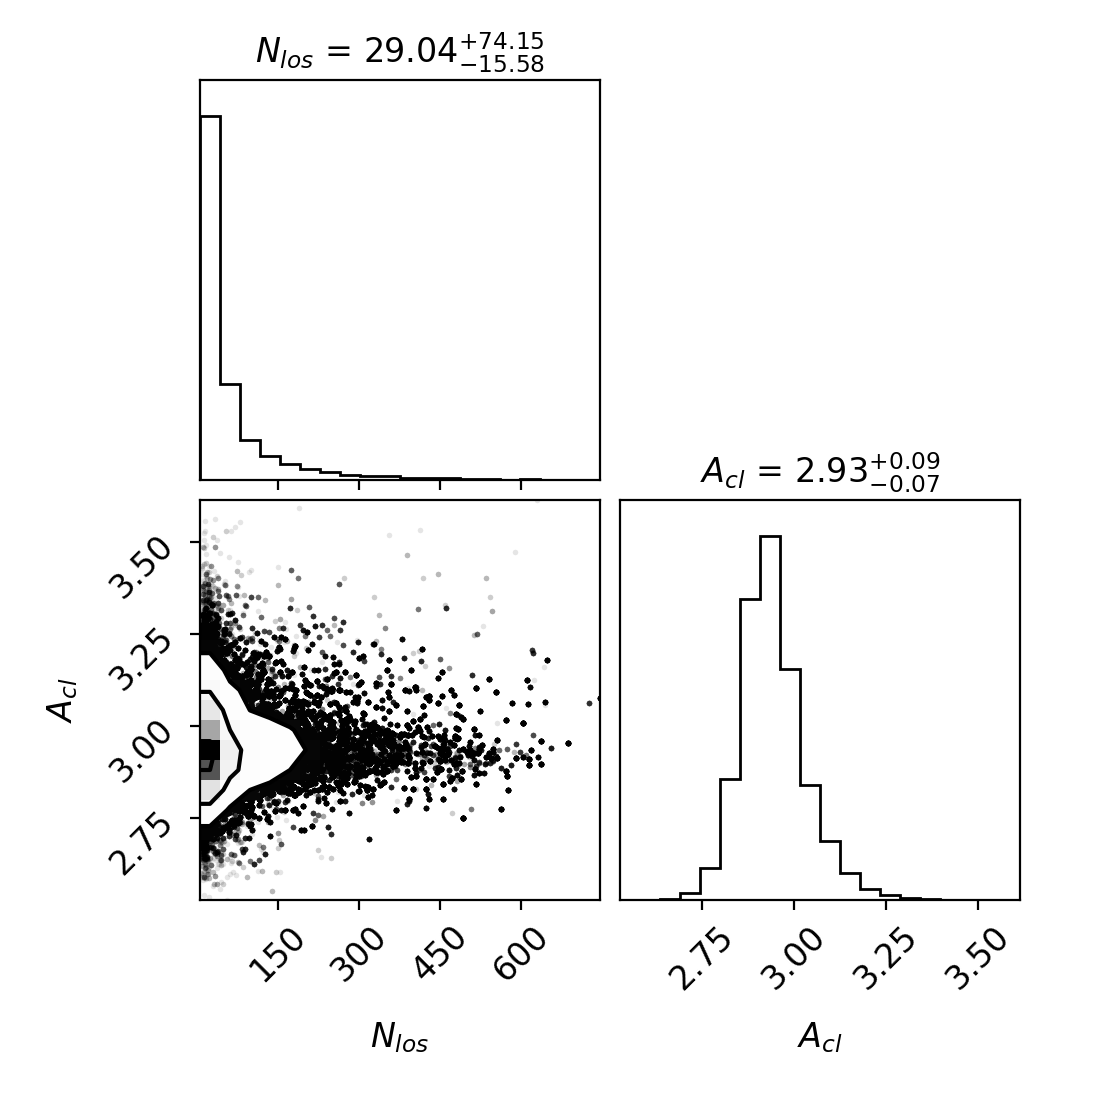
\includegraphics[scale=0.32]{figures/results/torus_only_prior_corner_plots/dynesty_0.1_1.0__priors_corner.png}
 \caption{Same as Figure~\ref{fig:tonlynopriorsparams}, but for the measured parameters \Nlos and \Acl not directly fit through dynamic nested sampling.}
 \label{fig:tonlynopriorsprior}
\end{figure}

\par In addition to the tunable parameters of the TORMAC model which have been directly fit by dynamic nested sampling, we also obtain measurements of other physically relevant quantities which are fixed for a given set of directly fit parameters. \Nlos is defined as the number of clouds on average intersected by rays originating at the central source and which radially extend to infinity and which pass through the torus distribution. \Acl is defined as the ratio of the surface areas of a single cloud relative to the inner surface area of the torus. For each of the posterior samples in Figure~\ref{fig:tonlynopriorsparams}, we calculate \Nlos and \Acl. For the anisotropic illumination case of the torus only model grid, we represent the samples from the estimated posterior distributions of \Nlos and \Acl as a corner plot in Figure~\ref{fig:tonlynopriorsprior}. The peak of posterior values for \Nlos and \Acl are very large, meaning that this torus distribution is optically thick and has very few clouds which are directly illuminated.
% \par In the top right panel of Figure 1, the volume filling factor (\vff), shown in log, is tightly constrained, with most samples ranging between 0.6\% and 0.3\% of the torus’ volume containing clouds. In the left panel of the second row, the radial cloud distribution (\p) is also tightly constrained around \p = 1. In the center panel, the inclination of the torus is also constrained to between approximately $57\degree$ and $67\degree$ (moderately inclined). In contrast, the right panel of the second row corresponding to the radial extent of the disk (\Y), is unconstrained as most samples tend to favor models at the lower bound of the parameter space ($Y \simeq 10R_d$) explored. Similarly, in the bottom left panel, the angular width of the torus (\sig) is also unconstrained, with most samples also favoring the lower bound of the parameter space (\sig $\simeq 5\degree$). \zach{want to do something like above with all other grid. Give specific and general info. want to format it sorta like X is Y+-Z, which is very constrained.}
% \par Both parameter estimations generally favor a compact (low \Y), thin (low \sig), torus with clouds taking up of order 0.1\% to 1\% of the torus volume (moderate \vff). They also favor a moderately inclined torus with the clouds somewhat centrally distributed in volume (\p $\approx 1$). The results from a torus only dust distribution showed that some of our parameters did not converge and favored the lower edge of the explored parameter space (notably \Y and \sig). Therefore, the models with a torus only component are not sufficient to explain the observed light curves and we widened our parameter space by including a polar dust distribution in addition to the torus. \zach{this is not WHY the models cannot explain the observed light curves, it is that there is a large amount of systematic error in our lightcurve still! Would be good to quantify the goodness of fit (we can do this)}


% \begin{figure}
%  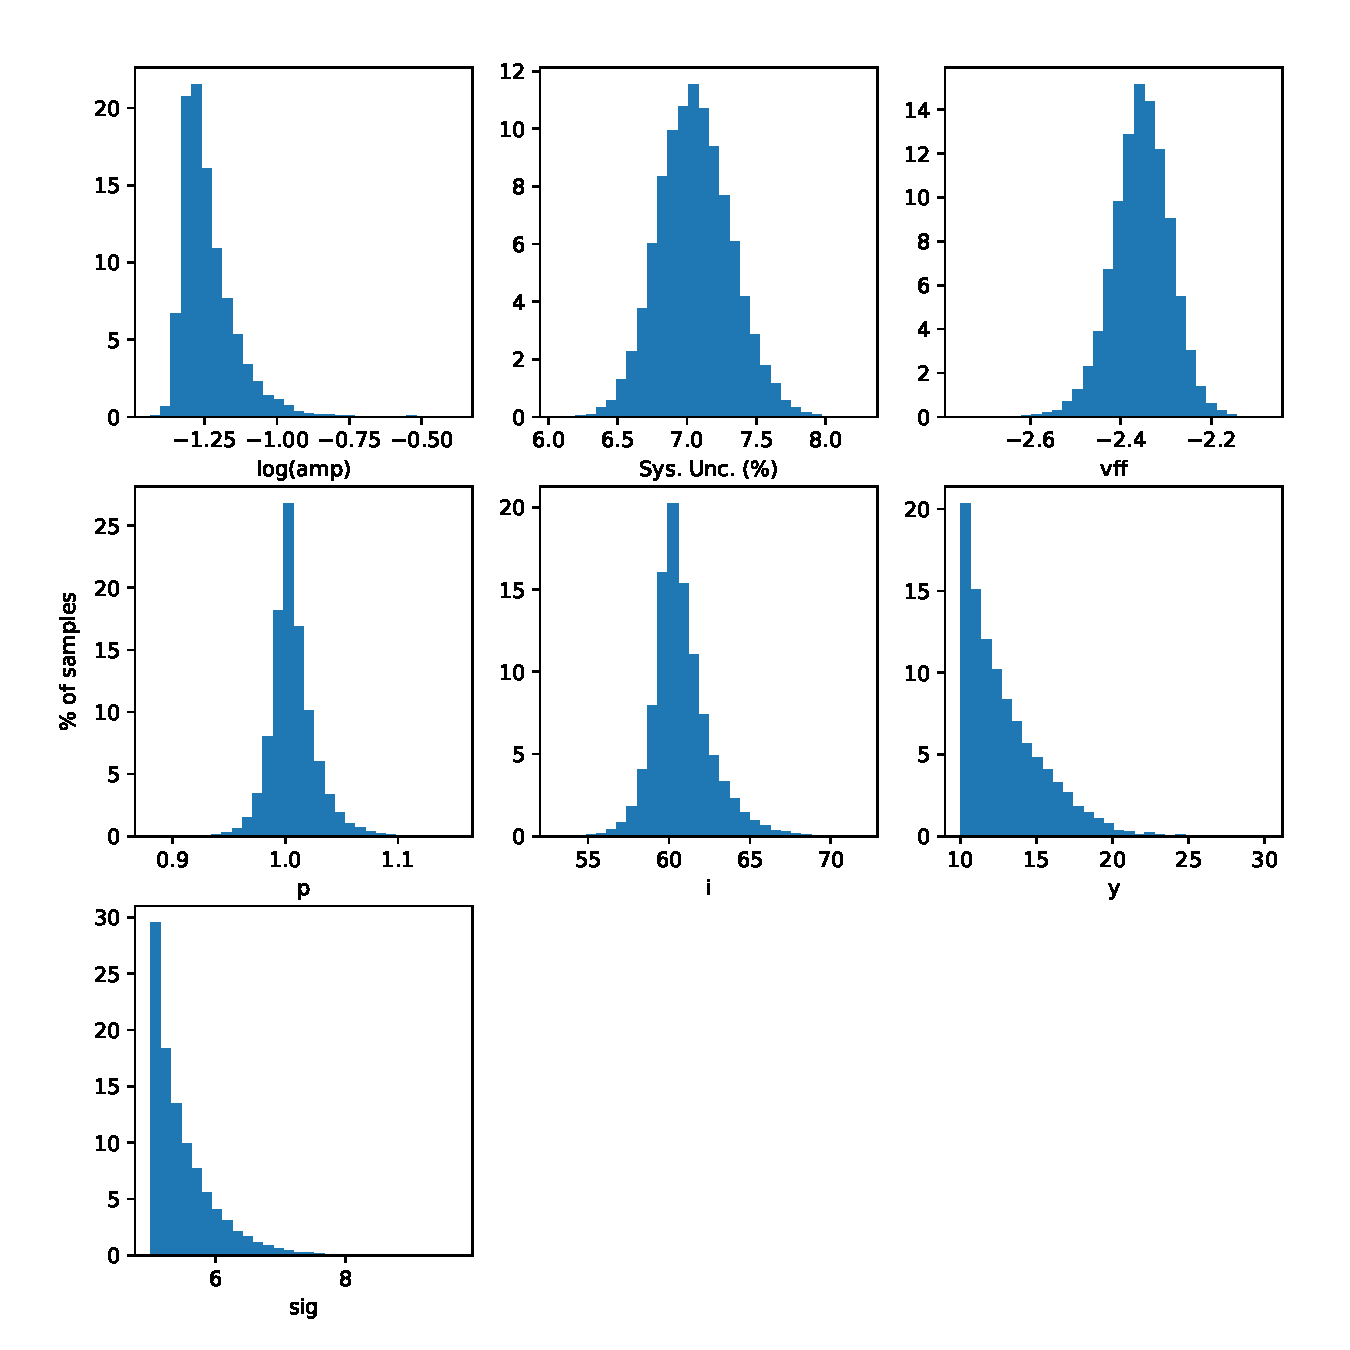
\includegraphics[width=\columnwidth]{G1CCA}
%  \caption{Posterior distribution generated by iterating tormacFit on the isotropic models from the initial torus only grid of models. Bar height corresponds to posterior probability. log(amp) and Sys. Unc. (\%) represent the free parameters introduced in Section~\ref{sec:tormacFit}, while the remaining panels enumerate all of the free parameters of the grid (see Table~\ref{tab:torus_only_params}). \zach{Why only showing isotropic?}}
%  \label{fig:torus_only}
% \end{figure}

% \subsection{Introduction of Polar Dust} %Grid 2
% \label{sec:introduction_of_polar_dust}

% \par In our second model set, we explore a dust distribution with both torus and polar dust components. One of the largest challenges with sampling the torus and polar dust parameter space is that many more degrees of freedom are introduced. We choose to reduce the number of free parameters by equating the relevant polar parameters to the equivalent torus parameters. For instance, in Table~\ref{tab:prop_polar_params}, \p/\ppol, \Y/\Ypol, \sig/\sigpol, and \vff/\vffpol have been paired, reducing the number of free parameters from 11 to 7. While we do not necessarily expect these parameters to be this correlated in AGN, this model grid is an initial attempt to introduce polar dust into our parameter estimation without adding too many degrees of freedom at once.

% Irrelevant now since not showing this

% \par Similar to the previous torus only models, tormacFit was run for both the isotropic models and the anisotropic models, producing two different posterior distributions. In Figure~\ref{fig:torus_prop_polar}, we only show the posterior distribution results from the isotropic models. \zach{Why?}
% \par Compared to the posterior distributions shown in Figure~\ref{fig:torus_only}, adding the proportional polar dust distribution resulted in a larger but more centrally located cloud distribution (lower \p \& \ppol, higher \Y \& \Ypol), a lower density (low \vff \& \vffpol), and higher inclinations (edge on) being favored. These models also support larger opening angles. \zach{Should I expand the best fit ranges for all of the grids or make them all like this?}
% \par Despite the introduction of a polar dust distribution, \sig, and now \inc, \vff, and \open are now unconstrained, with most models favoring edge of the explored parameter ranges. \zach{particularly dont like saying "most models favor the edge" can say this differently} We therefore determine that a torus and wind distribution with each of their respective parameters tied in value to each other is not sufficient to determine a unique, physically realistic fit to the data. Next, we explore varying more parameters of the polar dust structure.
% \par In the next set of models, we vary the polar dust structure parameters while holding the torus structure fixed. Table~\ref{tab:tori} shows the parameters of the grids of models were generated for each of the two fixed tori examined. The two torus configurations were determined from the peak of the posterior distributions of the previous model grids. The wind parameter values match the parameter values examined in the previous set of models. In addition, we add another free parameter, the cloud fraction, defined as \clfrac, corresponding to the fraction of clouds present in the torus versus the wind distributions. In the previous model grids, we adopted a standard of 67\% of the clouds in the torus, and 33\% of the clouds distributed equally between the top and bottom sections of the polar bi-cone. A cloud fraction of 1 represents all of the clouds residing in the torus, while a cloud fraction of 0 represents placing all of the clouds in the polar bi-cone. \zach{isnt this already in the code review?}

% \par Both posterior distributions, Figure \ref{fig:G3T1A} ("Torus 1") and Figure \ref{fig:G3T2A} ("Torus 2"), were generated using tormacFit by the same method as the previous model grids. We find that the wind distributions for both torus configurations vary significantly from the "proportional" parameter values tested before. In particular, Torus 1 shows significant bimodality in its inclination posterior distribution, favoring both lower, moderate inclinations (\inc $\approx 30$) as well as higher inclinations (\inc $\approx 60$). This bimodal degeneracy can be seen across multiple parameters. For both torus configurations, but especially Torus 1, more of the posterior samples fall within the parameter space. Still, \open (Torus 1 \& 2) as well as \vffpol, \Ypol, and \clfrac (Torus 2) favor the edge of the parameter space. Despite using a torus based on the peak of the previous model grid's posteriors, the modification of Torus 2's wind modified the most favored inclination from completely edge on to a more moderate inclination.
% \par Generally, the most samples across both posterior distributions favor an extended wind (roughly 10 times larger than the torus for Torus 1, and roughly twice as large as the torus for Torus 2) and a moderately centrally located polar cloud distribution (\ppol $\approx 0$). Torus 1's wind is better constrained, demonstrated by the narrower peaks in multiple parameters across the posterior distributions. Both winds favor a large fraction of the clouds residing in the wind.

\subsection{Variable Torus and Polar Dust Models}
\label{sec:parameter_estimation}

\begin{figure*}
 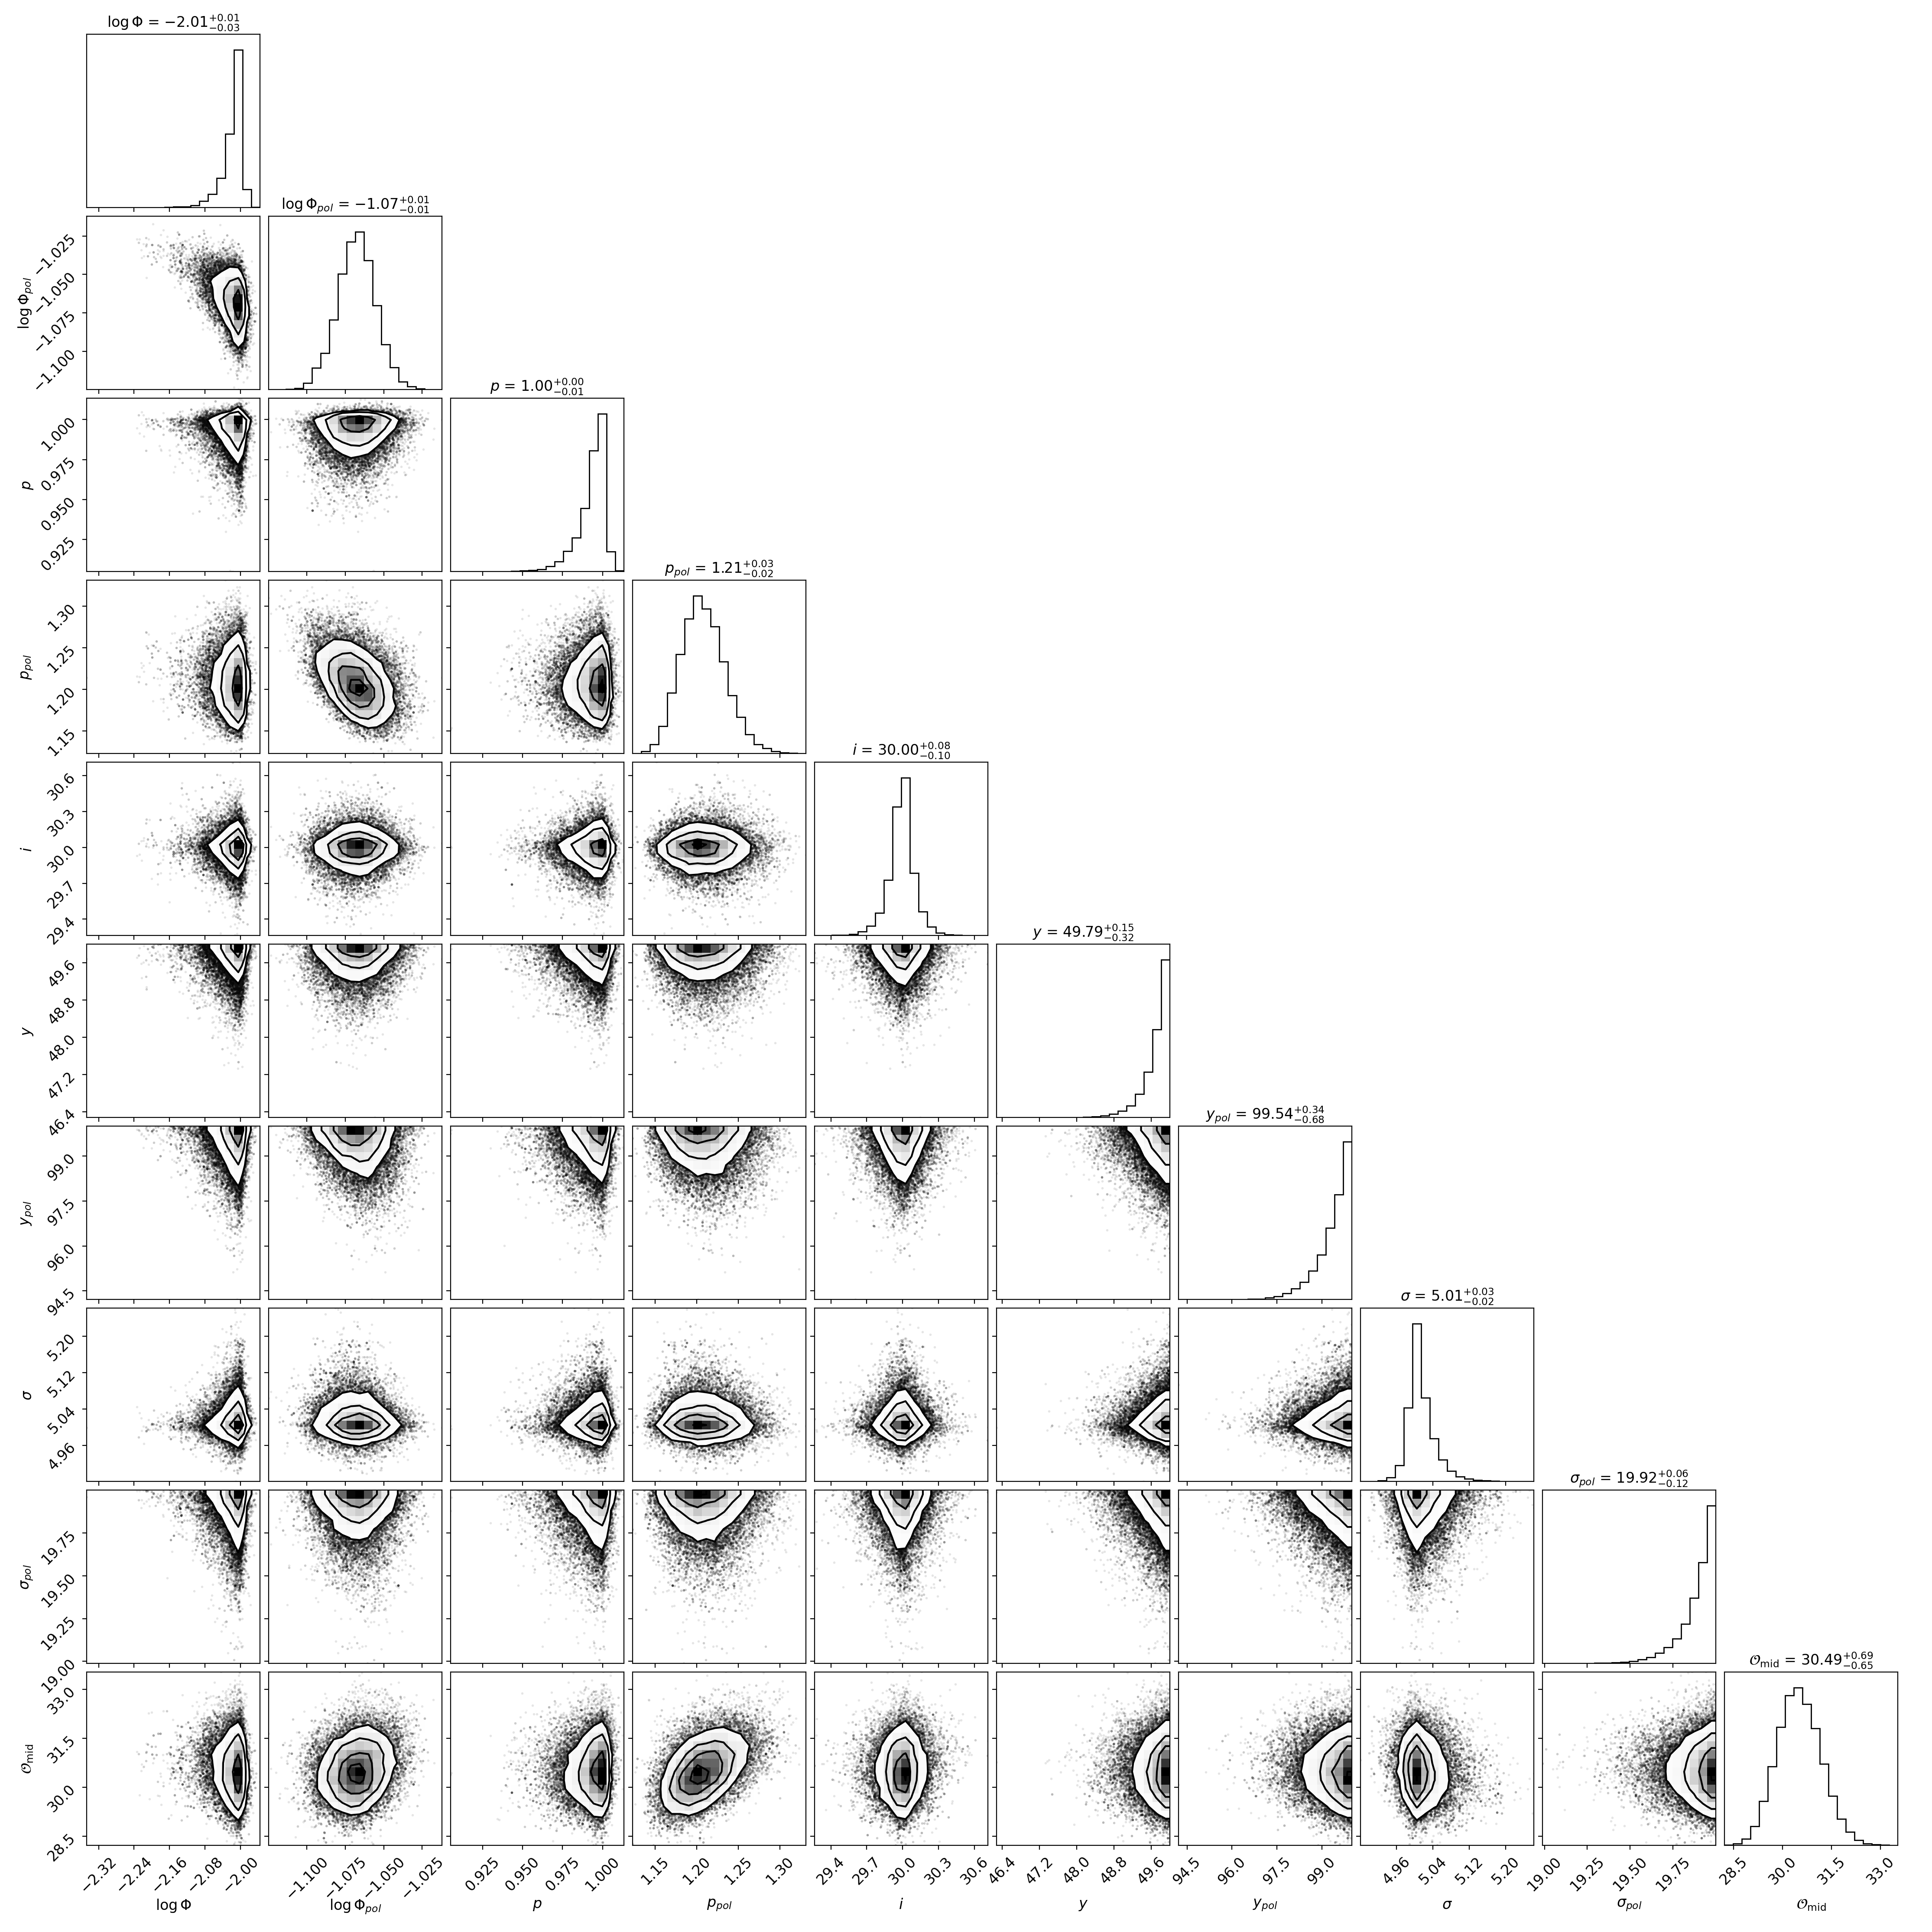
\includegraphics[scale=0.32]{corner_plots/dynesty_0.1_0.333__corner.png}
 \caption{\soft 0.1, \clfrac 0.333, no priors}
 \label{fig:nopriorsparams}
\end{figure*}

\begin{figure*}
 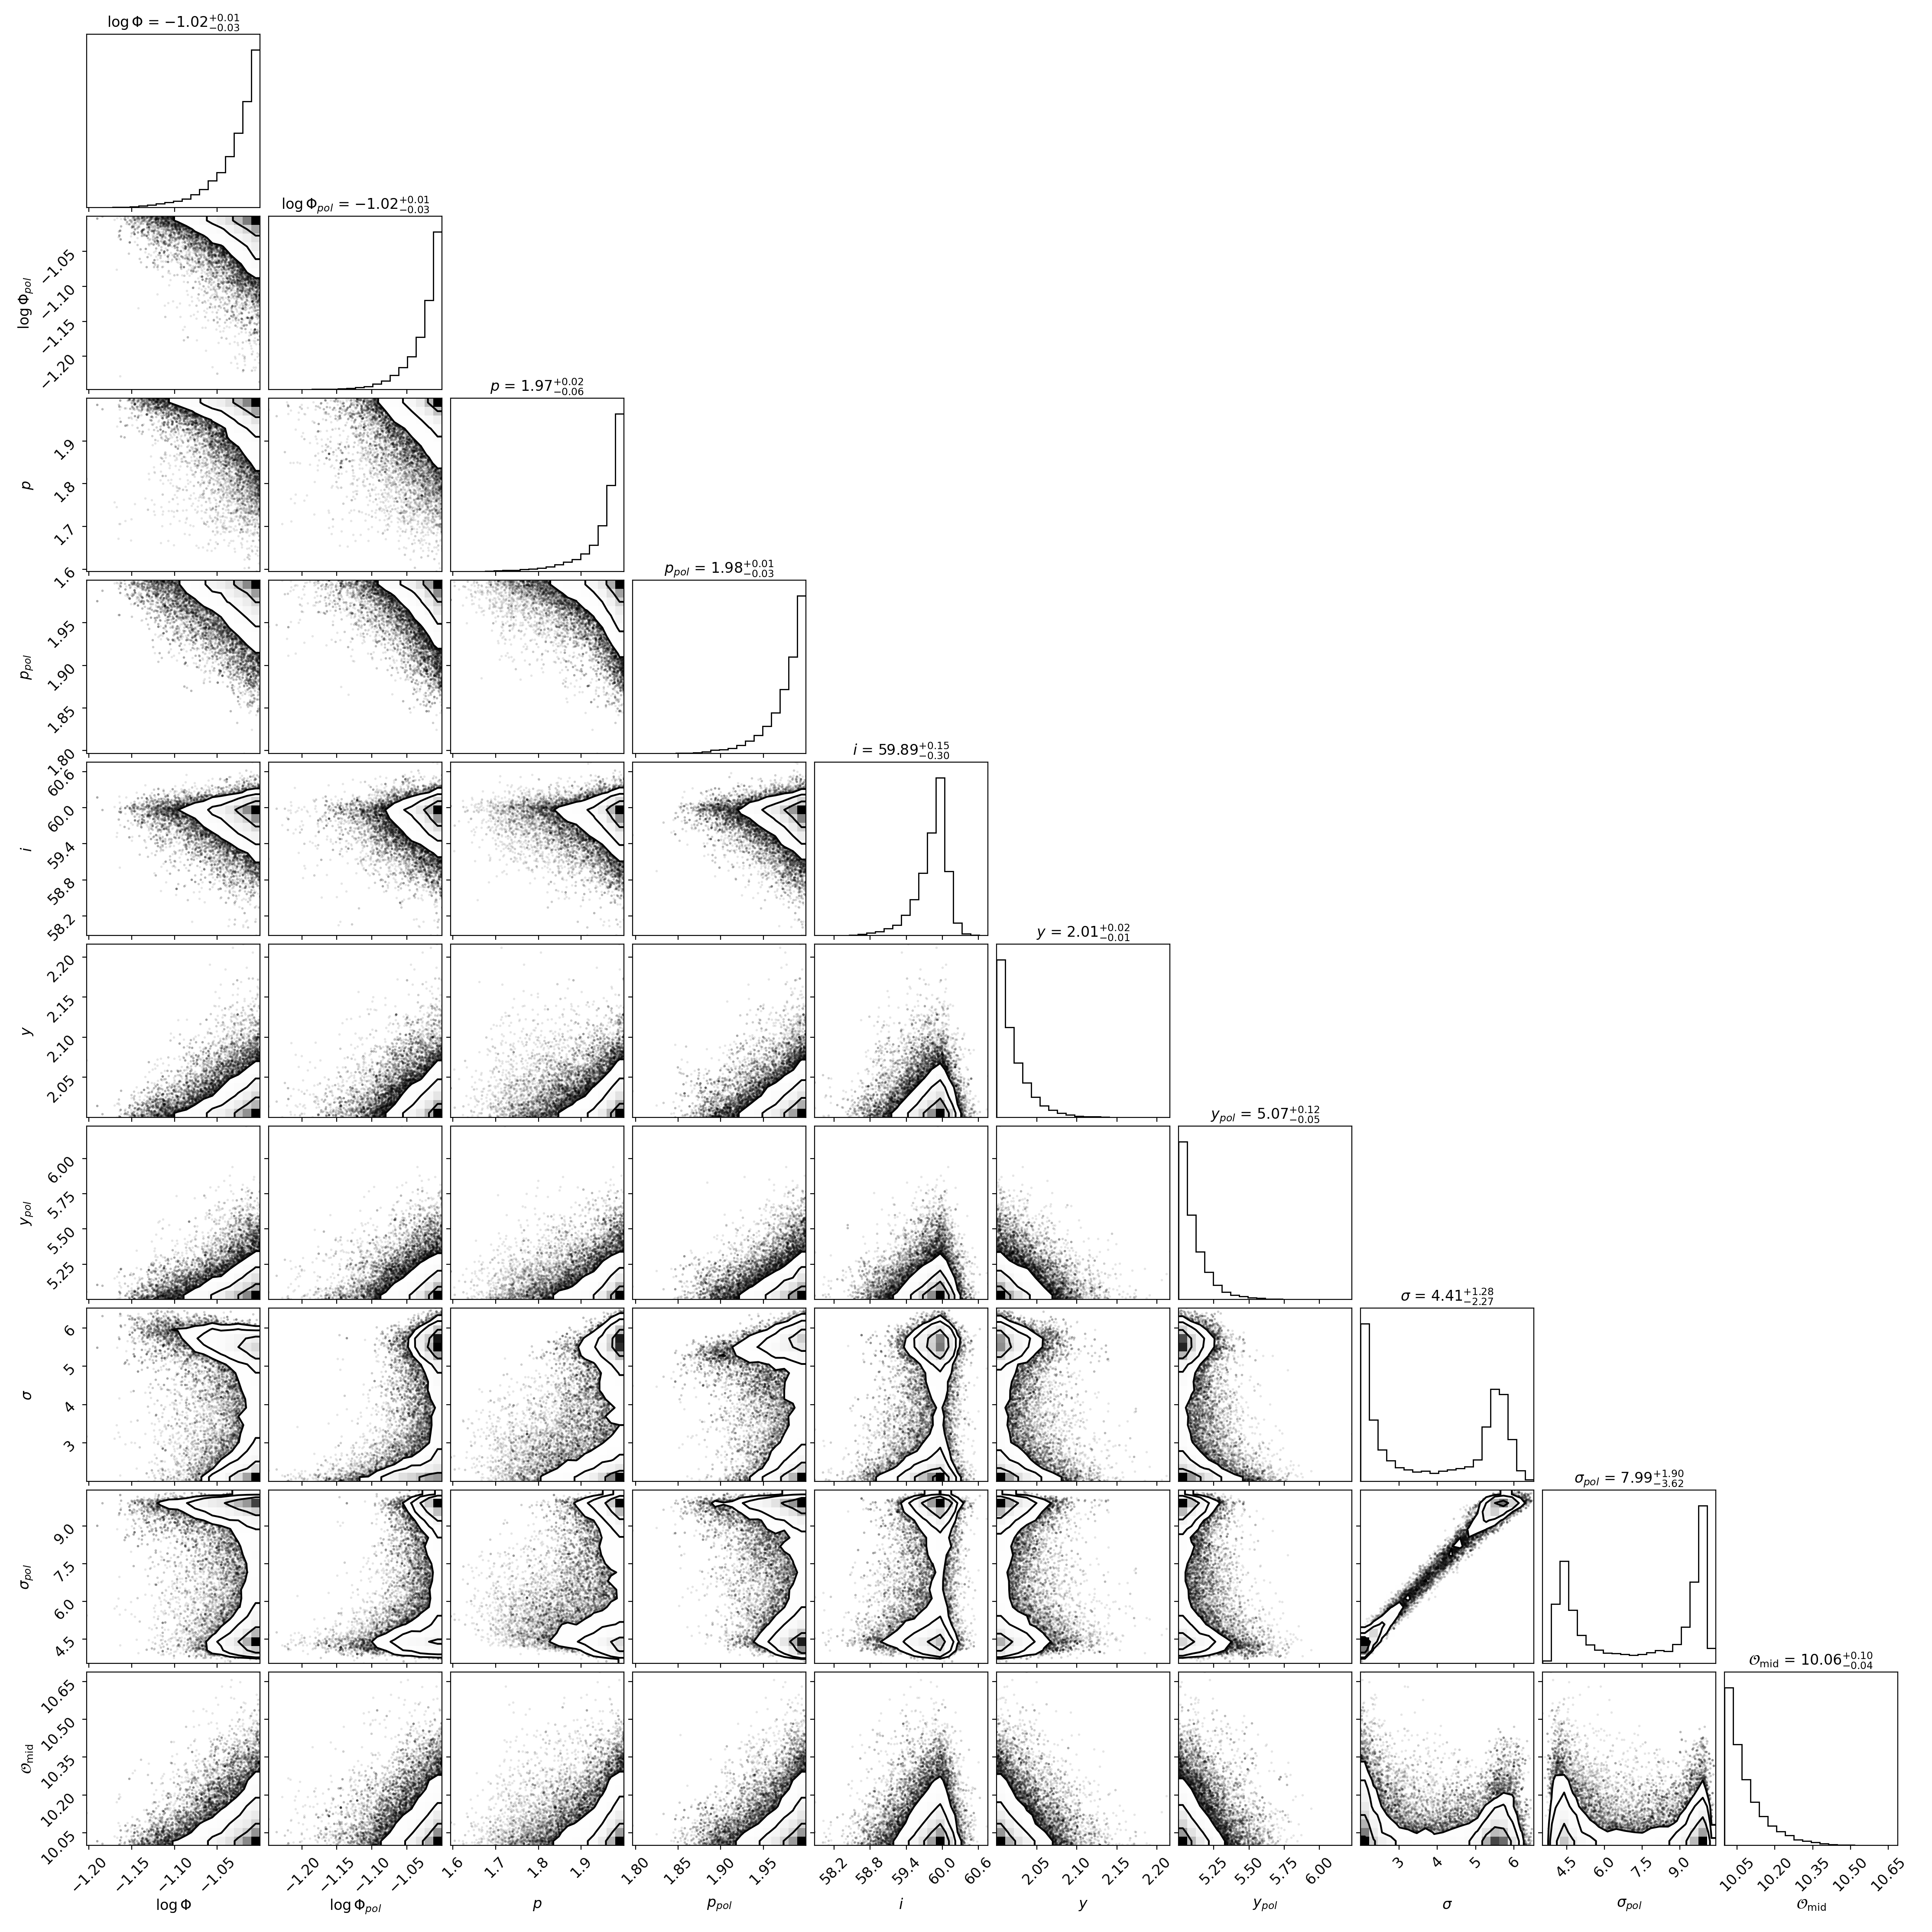
\includegraphics[scale=0.32]{corner_plots/dynesty_0.1_0.333_nlos_cloud_area_cloud_area_pol_cloud_size_ratio_corner.png}
 \caption{\soft 0.1, \clfrac 0.333, all priors}
 \label{fig:allpriorsparams}
\end{figure*}

\begin{figure}
 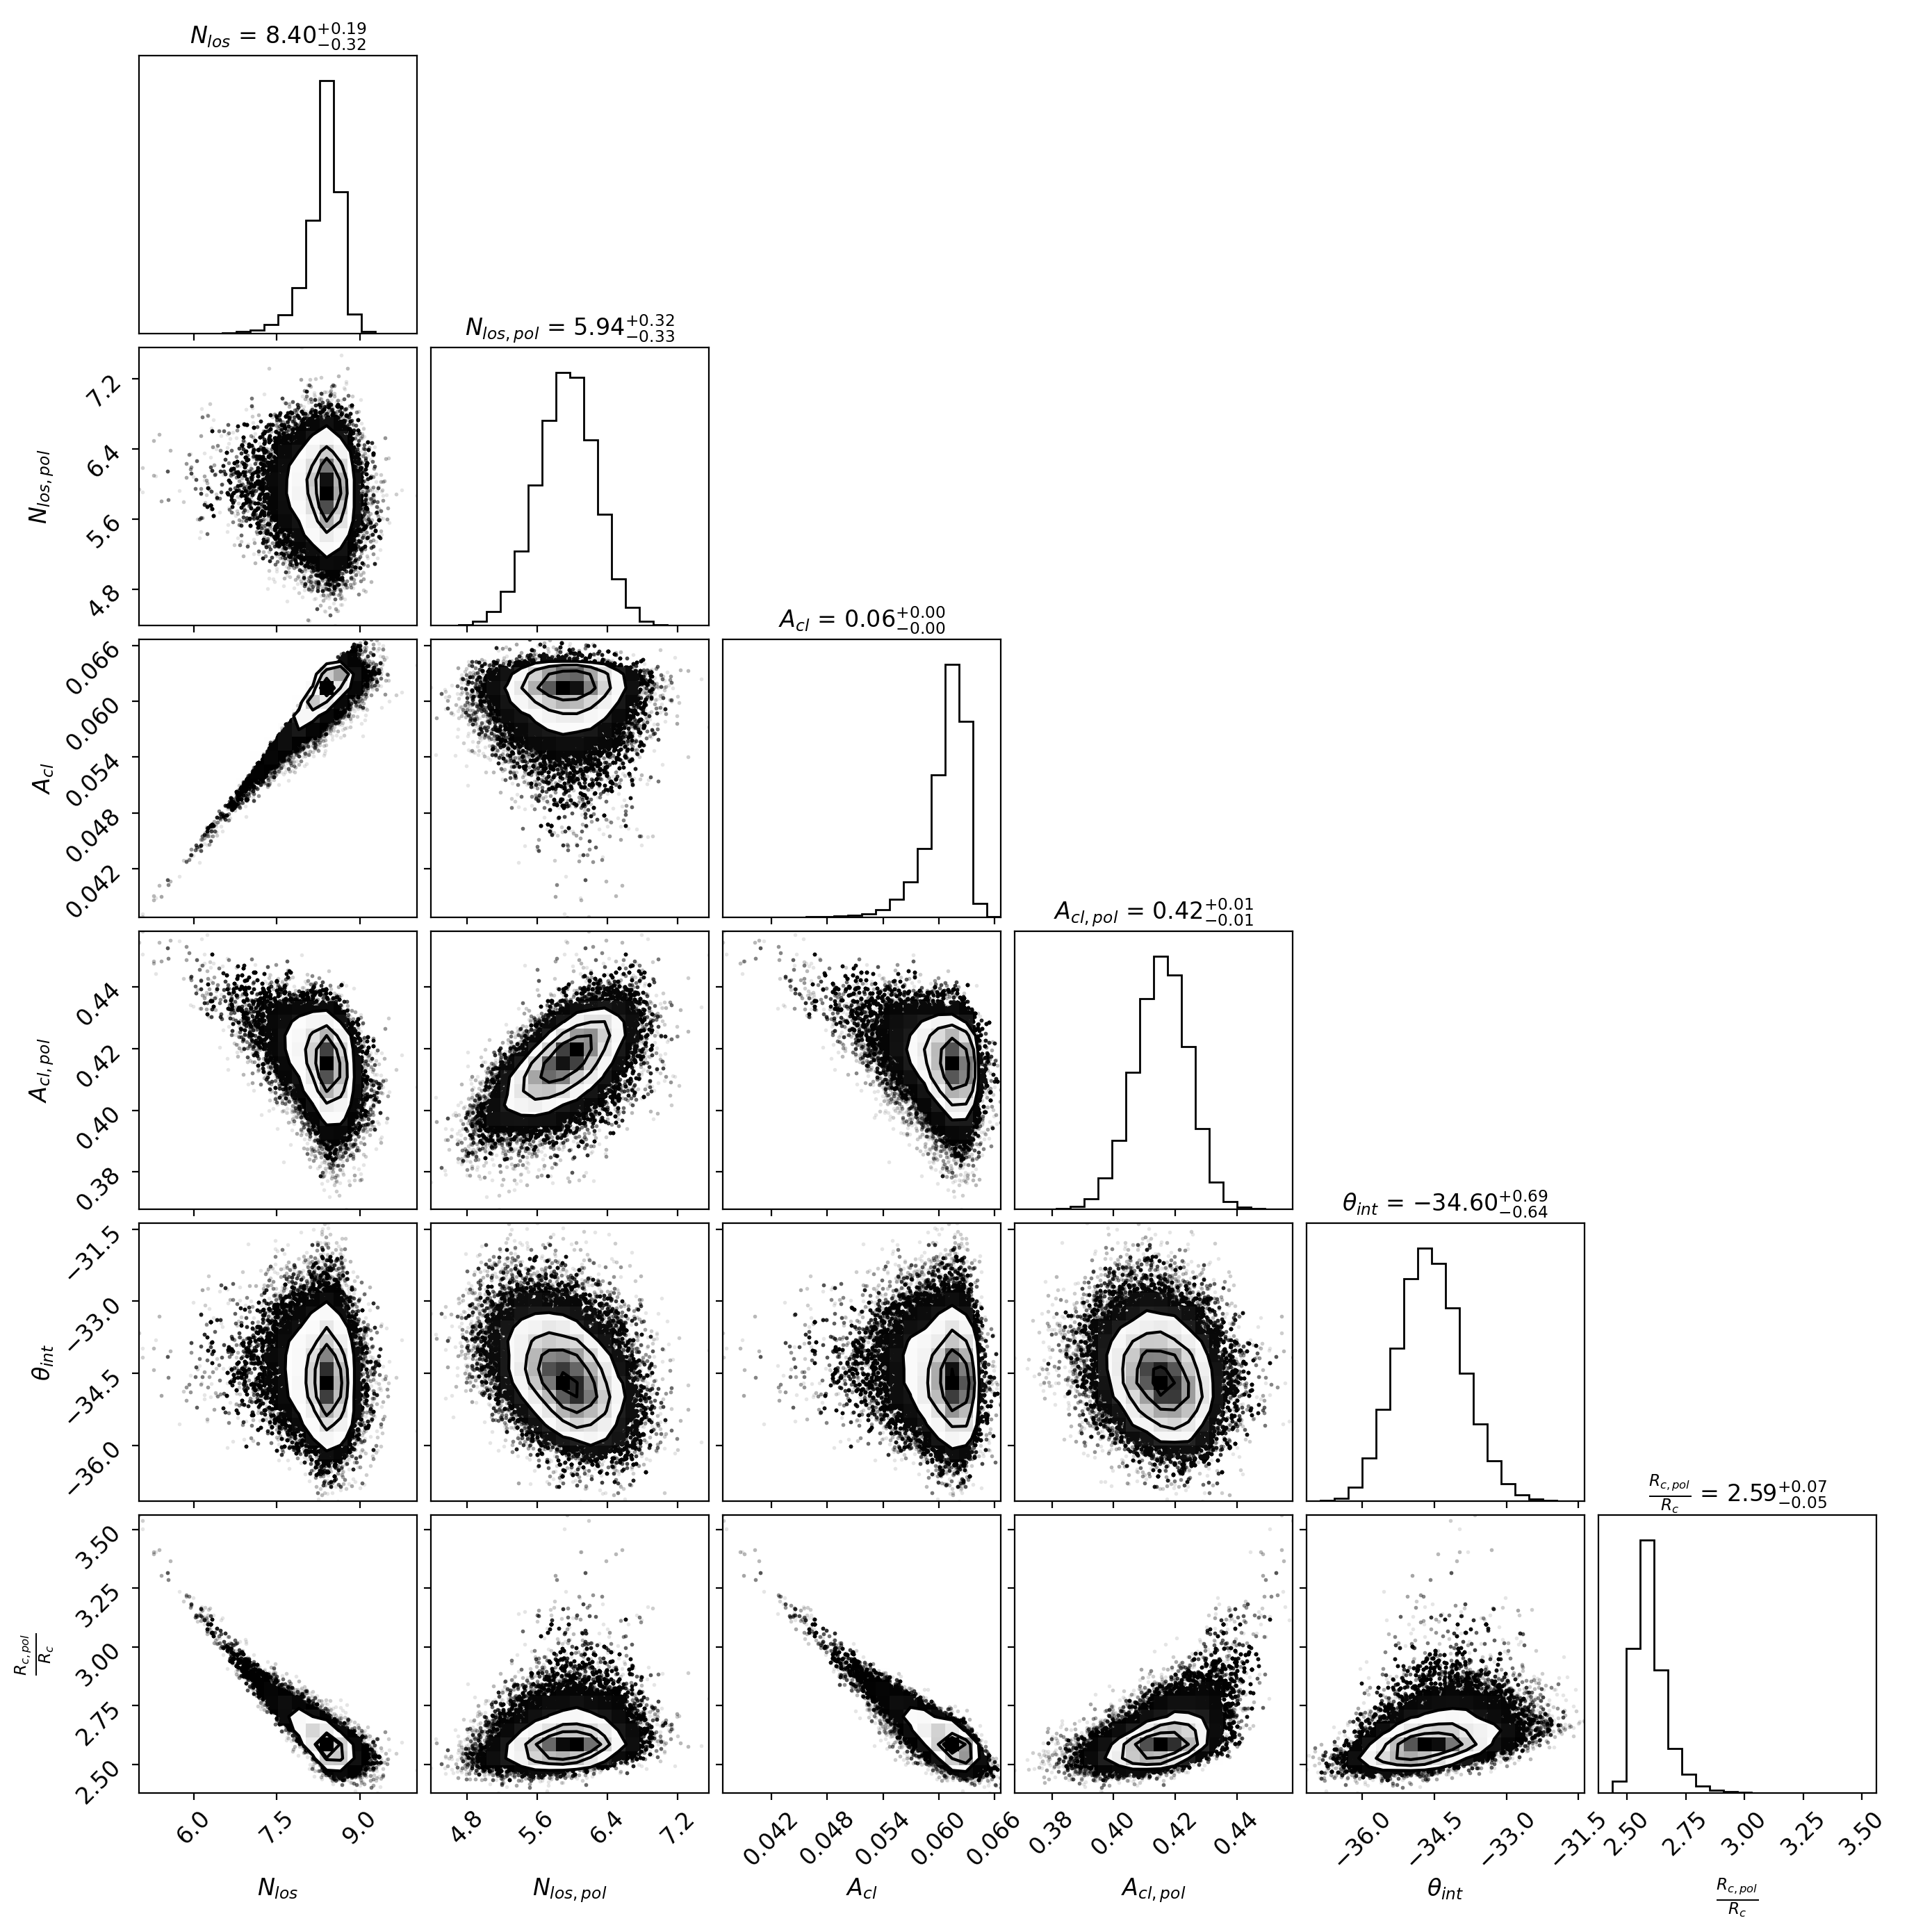
\includegraphics[scale=0.25]{prior_corner_plots/dynesty_0.1_0.333__priors_corner.png}
 \caption{\soft 0.1, \clfrac 0.333, no priors}
 \label{fig:nopriorsprior}
\end{figure}

\begin{figure}
 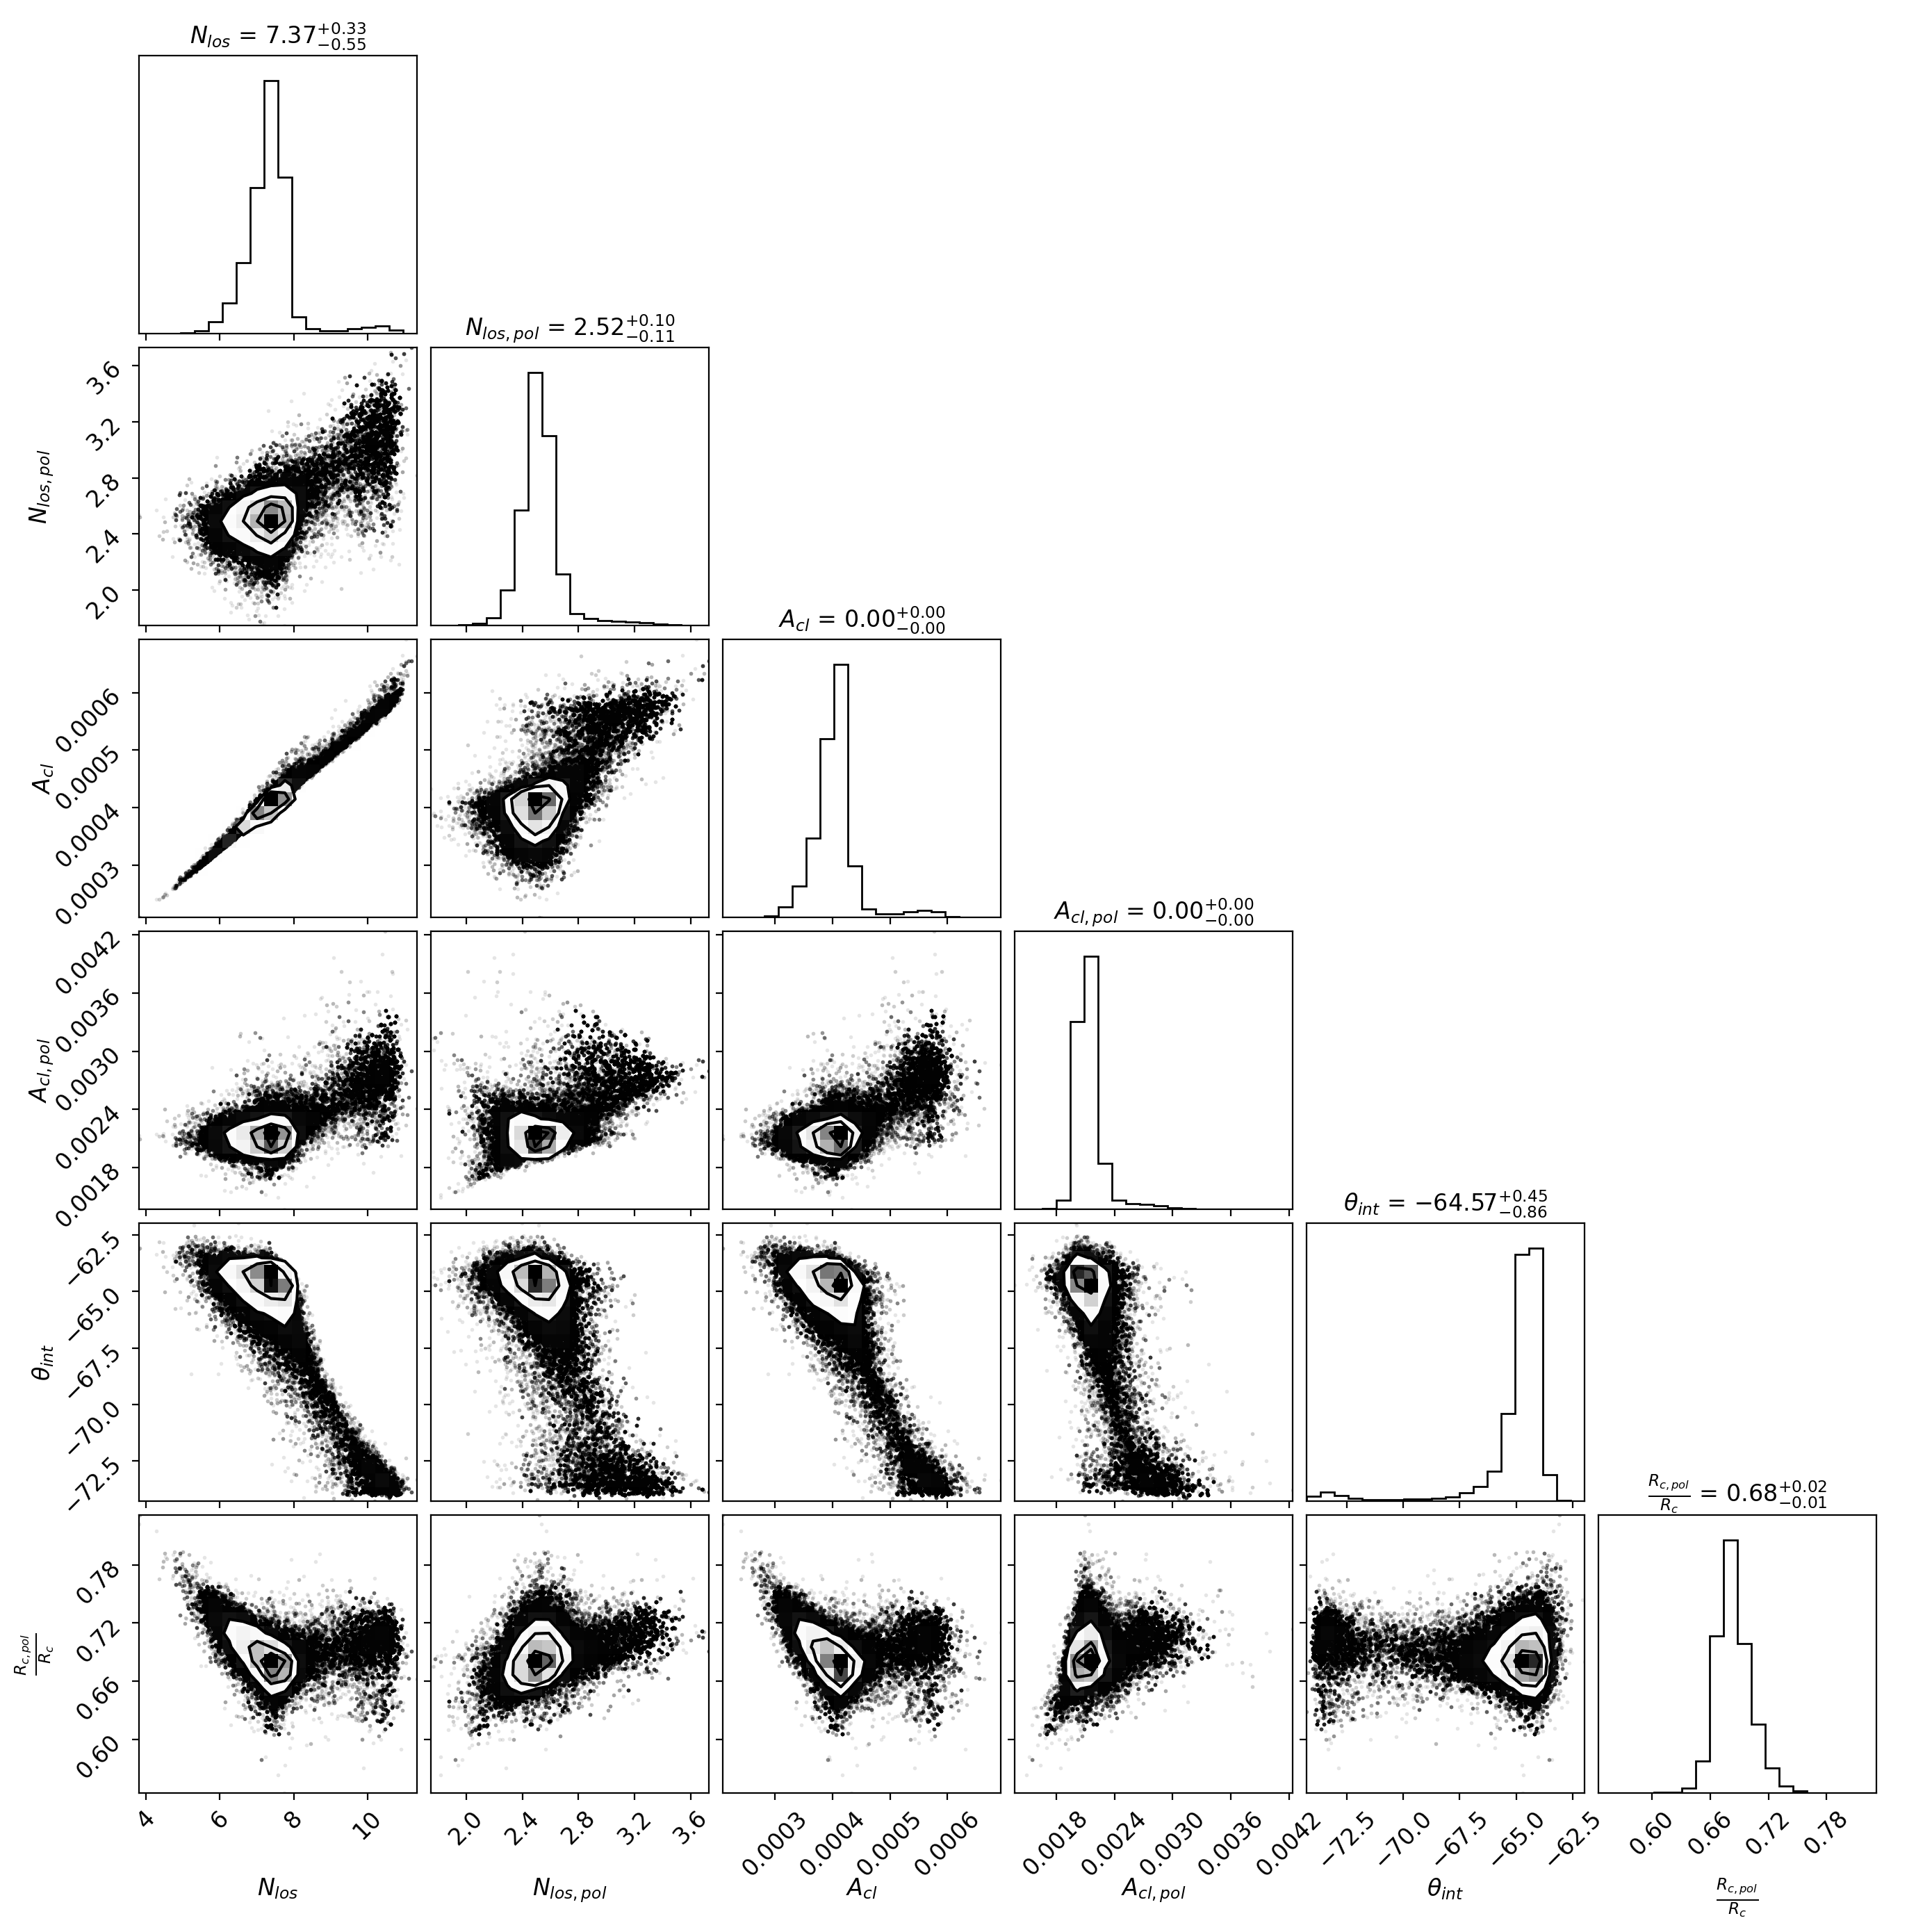
\includegraphics[scale=0.25]{prior_corner_plots/dynesty_0.1_0.333_nlos_nlos_pol_cloud_area_cloud_area_pol_cloud_size_ratio_priors_corner.png}
 \caption{\soft 0.1, \clfrac 0.333, all priors}
 \label{fig:allpriorsprior}
\end{figure}

%Reserving saying which grid is "better" for the discussion
% In Section~\ref{sec:torus_only_models},  we have shown that trying to limit the number of free parameters does not enable us to conclusively constrain the model fits to our data of NGC 3783.
\par While we initially chose to limit our model to only simulate the dust response from a single torus distribution, many AGN, including NGC 3783, have been shown through interferometry to also have extended warm dust IR emission perpendicular to the torus. Thus, we chose to include a simulated polar dust component in addition to a simulated torus component. This substantially increases the complexity of our model grid, resulting in roughly double the number of free parameters. Therefore, we choose to generate fewer TORMAC models at extreme (and not generally not physically supported) parameter values. First, we limited the inclination to be \inc $< 75\degree$, since for \inc $> 75\degree$ NGC 3783 would not have been able to be reverberation mapped. Additionally, we chose to not explore models beyond \Y = 100 due to the unphysically large clouds that the \Y $>50$ models produce and that these models have never been favored in the previous posteriors. Gleaning information from the torus only model, we also chose to decrease the minimum \Y value examined from 10 to 2. To limit numerical noise from having discrete clouds in our model, we chose to double the number of simulated clouds in the TORMAC models from 50000 to 100000, in order to keep the number of clouds in each distribution of order equal to the torus only case. To examine the effect that the number of clouds in each distribution has on the resulting light curve and posterior distribution, we, in addition to still evaluating both the isotropic and anisotropic illumination cases, now also evaluate separate grids with 1/3 of the simulated clouds being placed in the torus (\clfrac $= 0.333$) and 2/3 of the simulated clouds being placed in the torus (\clfrac $= 0.667$). This results in a total of four cases. As with the torus only grid, all parameter values are evaluated on a regular grid with grid points enumerated in Table~\ref{tab:params}. 

%Discussion! Can talk about this differently
% \par Of particular interest for constraining the dust morphology of NGC 3783 are models which satisfy observational constraints.  
% \par We find that regardless of choice of either isotropic or anisotropic illumination or modifying the cloud fraction, our estimated maximum likelihood model has clouds...
\par Of the four cases we evaluate, we choose to only show corner plots for the isotropic case with 1/3 of the clouds being placed in the torus dust distribution, but we enumerate the best fit parameters and associated $1\sigma$ errors for all four cases in Table~\ref{tab:best_fit}. 

\par We also used Dynesty to perform dynamic nested sampling on various subsets of the overall prior space. We do this to better understand how our estimated maximum likelihood model light curve and associated posterior distributions are affected by choice of several observational constraints.


\par Posteriors of the first set of models which vary both the torus and wind parameters independently. For this set, we choose to visualize both the 1d and 2d posteriors. 2d posteriors are able to show the relationships between parameters, as opposed to just their best fit. Down a column or across a row keeps one of the parameters constant while varying the other parameter. The 1d posteriors are the grid space where both of the parameters are the same. Contour lines for 0.5,1,1.5, and 2 sigma are shown.

\par As can be seen in Figure~\ref{fig:G4_corner_plot}, this model set tends to favor a very compact, moderately centrally dense, highly inclined torus with a significantly extended wind. We are able to constrain some of the parameters such as \p, \ppol, \inc, \Ypol, while other parameters remain unconstrained (\Y, \sig,\sigpol, \vff,\vffpol, and open). Due to the interesting behavior (especially \inc versus open) at large opening angles and \textbf{sigma pol}, the favoring of small \vff values, and the large gaps between some of our parameters, we adjusted and re-modeled NGC3783 using altered parameter values, and adding additional "inbetween" models to better explore the parameter space around the peak of the posteriors. The parameter values for this new set are enumerated in Table~\ref{tab:pe2}, and this set now contains about a million modeled response functions.

\par This expansion resulted in very few alterations to the best fit parameters, favoring very similar values to the previous set of models. 
%[I'm going to stop here because this is really up to the point where I am right now, without going into analysis.]